% !TeX spellcheck = en_GB
% \begin{figure}[t]
% 	\centering
%     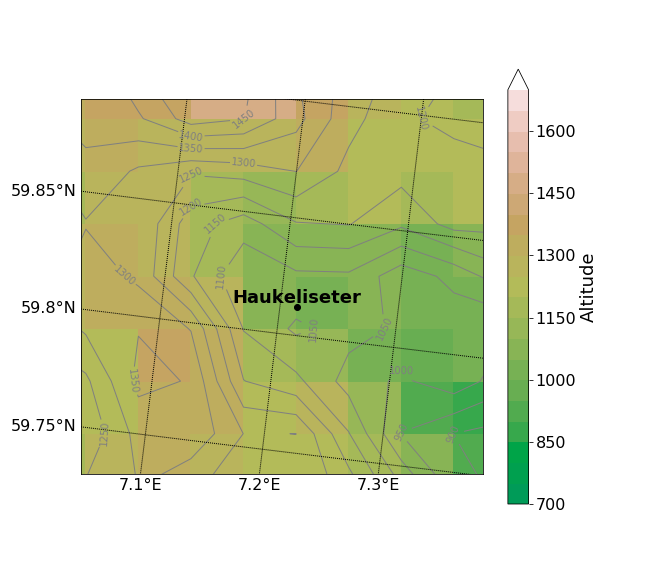
\includegraphics[trim={.3cm 2.2cm 1.8cm 2.4cm},clip,width=\textwidth]{./fig_Norway/MEPS_elevation_Haukeli}
%         \caption{}\label{fig:meps:site}
% \end{figure}

\begin{wrapfigure}{r}{0.55\textwidth}
	\vspace{-\normalbaselineskip}
	\centering
	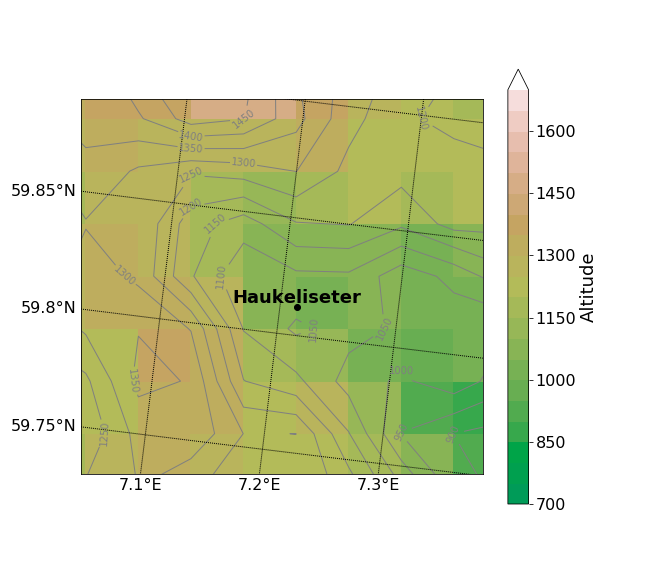
\includegraphics[trim={.3cm 2.2cm 1.8cm 2.4cm},clip,width=0.54\textwidth]{./fig_Norway/MEPS_elevation_Haukeli}
	%	\vspace{-10pt}
	\caption{Representation of the topography around measurement site Haukeliseter in MEPS. Contours and shading present the elevation of the grid cells.}\label{fig:meps:site}
	\vspace{-\normalbaselineskip}
\end{wrapfigure}